\documentclass[tikz,border=5pt]{standalone}
\usepackage[T1]{fontenc}
\usepackage{lmodern,amsmath,amssymb}
\usetikzlibrary{arrows.meta,calc,positioning,fit,backgrounds,shapes.geometric,matrix,decorations.pathreplacing,patterns}
\definecolor{ink}{gray}{0.08}
\definecolor{wash}{gray}{0.965}
\definecolor{soft}{gray}{0.45}
\tikzset{box/.style={draw=ink,line width=.65pt,fill=white,align=center,inner sep=4pt,outer sep=0pt,font=\small},flow/.style={draw=ink,line width=.65pt,-{Latex[length=1.8mm,width=1.3mm]},rounded corners=2pt},annotation/.style={font=\scriptsize,text=soft,align=center},groupbox/.style={draw=soft,dashed,line width=.45pt,fill=wash}}
\begin{document}
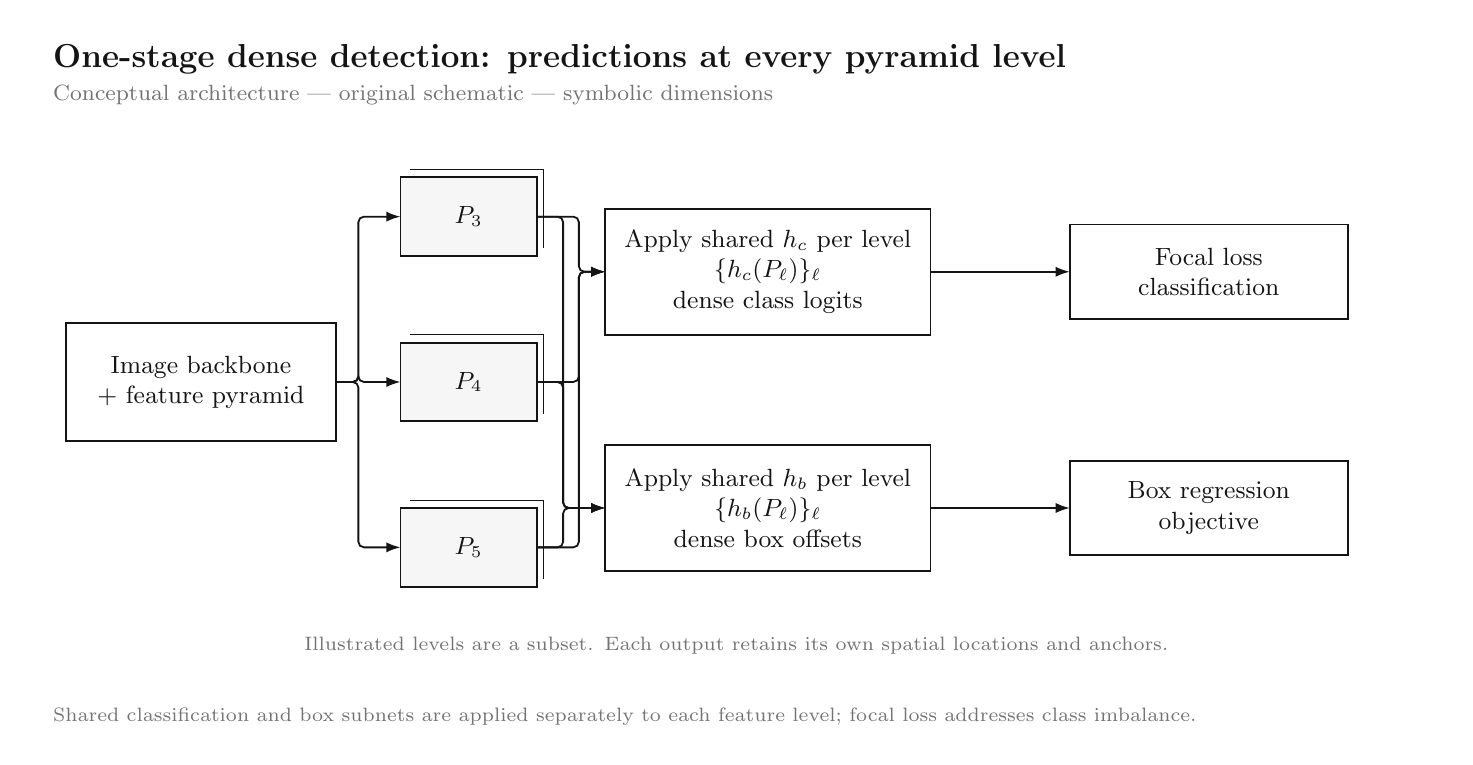
\begin{tikzpicture}[x=1cm,y=-1cm,font=\rmfamily,text=ink]

\path[use as bounding box] (0,0) rectangle (18,9);
\node[anchor=west,font=\large\bfseries] at (.2,.4) {One-stage dense detection: predictions at every pyramid level};
\node[anchor=west,font=\footnotesize,text=soft] at (.2,.85) {Conceptual architecture | original schematic | symbolic dimensions};
\begin{pgfonlayer}{background}
\end{pgfonlayer}
\node[box,minimum width=3.4cm,minimum height=1.5cm,text width=3.15cm] (back) at (2.2,4.5) {Image backbone\\+ feature pyramid};
\node[box,fill=wash,minimum width=1.7cm,minimum height=1.0cm,text width=1.45cm] (p3) at (5.6,2.4) {$P_3$};
\draw[ink,line width=.4pt] (4.85,1.7999999999999998) -- (6.549999999999999,1.7999999999999998) -- (6.549999999999999,2.8);
\node[box,fill=wash,minimum width=1.7cm,minimum height=1.0cm,text width=1.45cm] (p4) at (5.6,4.5) {$P_4$};
\draw[ink,line width=.4pt] (4.85,3.9) -- (6.549999999999999,3.9) -- (6.549999999999999,4.9);
\node[box,fill=wash,minimum width=1.7cm,minimum height=1.0cm,text width=1.45cm] (p5) at (5.6,6.6) {$P_5$};
\draw[ink,line width=.4pt] (4.85,6.0) -- (6.549999999999999,6.0) -- (6.549999999999999,7.0);
\node[box,minimum width=4.1cm,minimum height=1.6cm,text width=3.8499999999999996cm] (cls) at (9.4,3.1) {Apply shared $h_c$ per level\\$\{h_c(P_\ell)\}_\ell$\\dense class logits};
\node[box,minimum width=4.1cm,minimum height=1.6cm,text width=3.8499999999999996cm] (reg) at (9.4,6.1) {Apply shared $h_b$ per level\\$\{h_b(P_\ell)\}_\ell$\\dense box offsets};
\node[box,minimum width=3.5cm,minimum height=1.2cm,text width=3.25cm] (fl) at (15.0,3.1) {Focal loss\\classification};
\node[box,minimum width=3.5cm,minimum height=1.2cm,text width=3.25cm] (bl) at (15.0,6.1) {Box regression\\objective};
\begin{pgfonlayer}{background}
\draw[flow] (back.east) -- (4.2,4.5) -- (4.2,2.4) -- (p3.west);
\draw[flow] (back.east) -- (4.2,4.5) -- (4.2,4.5) -- (p4.west);
\draw[flow] (back.east) -- (4.2,4.5) -- (4.2,6.6) -- (p5.west);
\draw[flow] (p3.east) -- (7.0,2.4) -- (7.0,3.1) -- (cls.west);
\draw[flow] (p3.east) -- (6.8,2.4) -- (6.8,6.1) -- (reg.west);
\draw[flow] (p4.east) -- (7.0,4.5) -- (7.0,3.1) -- (cls.west);
\draw[flow] (p4.east) -- (6.8,4.5) -- (6.8,6.1) -- (reg.west);
\draw[flow] (p5.east) -- (7.0,6.6) -- (7.0,3.1) -- (cls.west);
\draw[flow] (p5.east) -- (6.8,6.6) -- (6.8,6.1) -- (reg.west);
\draw[flow] (cls.east) -- (fl.west);
\draw[flow] (reg.east) -- (bl.west);
\end{pgfonlayer}
\node[annotation,text width=14cm] at (9,7.85) {Illustrated levels are a subset. Each output retains its own spatial locations and anchors.};
\node[anchor=west,align=left,font=\scriptsize,text=soft,text width=17.6cm] at (.2,8.75) {Shared classification and box subnets are applied separately to each feature level; focal loss addresses class imbalance.};
\end{tikzpicture}
\end{document}
